% Use only LaTeX2e, calling the article.cls class and 12-point type.

\documentclass[11pt]{article}

\usepackage[round,semicolon]{natbib}
\usepackage{etoolbox}
\AtBeginEnvironment{quote}{\singlespacing\tiny}
% Use times if you have the font installed; otherwise, comment out the
% following line.

% added by SKH
%\usepackage{lineno}
%\linenumbers

\usepackage{times}
\usepackage{amssymb}
\usepackage{amsmath}

\usepackage[export]{adjustbox}

\usepackage{graphicx}
\graphicspath{ {images/} }

% for adjustwidth
\usepackage{changepage}

% The following parameters seem to provide a reasonable page setup.

\topmargin 0.0cm
%\oddsidemargin 2cm
%\textwidth 16cm 
\textheight 21cm
\footskip 1.0cm

\usepackage{newfloat}
\usepackage{amsmath}
\usepackage[labelfont=bf]{caption}
\usepackage{nameref}
\usepackage{rotating}
\usepackage{color}
\usepackage{float}
\renewcommand{\figurename}{{}}
\renewcommand{\thefigure}{{Figure \arabic{figure}}}

\renewcommand{\tablename}{{}}
\renewcommand{\thetable}{{Table \arabic{table}}}

\newfloat{suppfile}{thp}{losuppfile}
\renewcommand{\thesuppfile}{Supplementary file \arabic{suppfile}}
\floatname{suppfile}{}

\newfloat{suppfig}{thp}{losuppfig}
\renewcommand{\thesuppfig}{Supplementary figure \arabic{suppfig}}
\floatname{suppfig}{}

%
\newfloat{supptable}{thp}{losupptable}
\renewcommand{\thesupptable}{Supplementary table \arabic{supptable}}
\floatname{supptable}{}
%

\renewcommand{\theequation}{Equation \arabic{equation}}

\newcommand{\mutDNA}{\textbf{mutDNA}}
\newcommand{\mutvirus}{\textbf{mutvirus}}
\newcommand{\DNA}{\textbf{DNA}}
\newcommand{\virus}{\textbf{virus}}

\newcommand\skhcomment[1]{{\color{cyan}[#1]}}
\newcommand\jdbcomment[1]{{\color{red}[#1]}}


\usepackage{hyperref}
\hypersetup{colorlinks,citecolor=blue,linkcolor=blue,urlcolor=blue}
\hypersetup{colorlinks,citecolor=blue,linkcolor=blue,urlcolor=blue}

\usepackage{seqsplit}

\usepackage{array}
\newcolumntype{P}[1]{>{\raggedright\arraybackslash}p{#1}}

\title{Experimentally informed site-specific substitution models deepen phylogenetic estimates of the divergence of viral lineages} 

\author
{Sarah K. Hilton$^{1,2}$  and Jesse D. Bloom$^{1,2}$\\
\\
\normalsize{$^1$Division of Basic Sciences and Computational Biology Program,}\\
\normalsize{Fred Hutchinson Cancer Research Center, Seattle, WA 98109, USA}\\
\normalsize{$^2$Department of Genome Sciences, University of Washington, Seattle, WA}\\
\normalsize{E-mail:  jbloom@fredhutch.org.}\\
}


% Include the date command, but leave its argument blank.

\date{}

\usepackage{setspace}
\onehalfspacing


\begin{document} 

% Make the title.

\maketitle 


\begin{abstract}
\noindent  
Molecular phylogenetics is used to estimate the time since the divergence of modern gene sequences.
Such phylogenetic techniques often estimate substantially shallower divergence times than other methods.
For instance, in the case of viruses there is independent evidence that molecular phylogenetics can underestimate deep divergence times.  
This discrepancy is thought to be caused in part by inadequate models of purifying selection leading to branch-length underestimation.
Here we show that models informed by experimental measurements of purifying selection due to site-specific amino-acid preferences lengthen deep branches on phylogenies of influenza virus hemagglutinin.
This deepening of branch lengths is due to better modeling of the stationary state of the substitution models, and is independent of the branch-length-extension that results from modeling site-to-site variation in substitution rate.
The branch-length extension from experimentally informed site-specific models is similar to that achieved by other approaches that allow the stationary state to vary across sites.
However, the improvements from these site-specific models are limited by the inherent tension between the enhanced accuracy of accounting for site-specific amino-acid preferences and the fact that these preferences shift over long evolutionary times.
Overall, our work underscores the importance of modeling how site-specific purifying selection affects the stationary state when estimating deep divergence times. 
\end{abstract}

\clearpage

\section*{Introduction} 
\skhcomment{from JDB: what is the "age" of a virus? Maybe "divergence time of viral lineages"}
skhcomment{from JDB: what is the less than a million actually? "Old" is not the right phrase.}
Estimating the divergence time of viral lineages of a virus is essential to understanding its evolutionary history, including its emergence, spread, and past zoonoses. 
This estimation is commonly done using the concept a ``molecular clock" to transform the branch lengths of the viral phylogenetic tree into age in years. 
However, this molecular dating technique often underestimates the age of many viruses, including measles, foamy virus, and ebola \skhcomment{(citations)}, compared to other methods which are independent of the viral phylogeny. 
For example, SIV (the original source of HIV) is estimated to be less than a million years old based on the viral phylogeny \citep{sharp2000origins,wertheim2009dating,worobey2010island} but estimated to be several million years old based on the host tree or endogenous retroviral elements  \citep{compton2013host} \skhcomment{(other citations)}. 
Overall, there is a systematic and substantially large underestimation of of branch length on viral phylogenies. 
\skhcomment{long branches}

Branch length underestimation is due, in part, to strong purifying selection masking the evolutionary signal in the observed sequences. 
Purifying selection can lead to mutational saturation, where multiple unobserved, substitutions occur at a single site along a long branch and erase the divergence signal \citep{holmes2003molecular}.
Furthermore, proteins do not have equal preference for all amino acids at all sites, this evident by a simple visual inspection of a multiple sequence alignment. 
How many and which amino acids tolerated at each site of the protein generate a site-specific expected rate of change. 
Failing to account for these site-specific constraints will lead to branch length underestimation. 
\skhcomment{you will have mutational saturation no matter what - this is a separate, addressable issue?}
\skhcomment{talk about the high mutation rate in viruses?}

Substitution models that incorporate site-to-site rate variation have been developed to decrease the bias in long branch estimation. 
The most common strategy is to allow a single rate-controlling parameter to vary according to some statistical distribution, such as a $\Gamma$-distributed $\omega$ (~dN/dS) \citep{yang2000codon}. 
This flexibility in the value of $\omega$ accounts for the site-to-site rate variation by allow some sites to have a higher dN/dS value than others. 
While this modification is simple and only requires the addition of one extra parameter, it does not describe site-specificity in its stationary state. 
That is, at evolutionary equilibrium, this model still assumes that each site in the protein evolves identically.  

An alternative approach is to model the site-specific amino-acid frequencies explicitly, such as those models in the mutation-selection family \citep{halpern1998evolutionary}. 
In these models, each amino-acid at each site in the protein is described by its own parameter and these differences are reflected in the stationary state of the model. 
The rate of change at a given site is controlled by these amino acid profiles and can now vary from site to site, as expected based on observations in nature. 
Importantly, these rate variations are not constrained to an arbitrary statistical distribution but by parameters with a direct biological interpretation. 

Mutation-selection models are presumably more biologically relevant but pose more practical challenges than the $\Gamma\omega$ models. 
These models are highly parametrized with 19 free parameters (the 20 amino acid preferences are constrained to sum to one) per site leading to thousands of parameters for the length of a normal protein. 
One way to avoid overfitting is to implement the model as a mixture model in either a bayesian \citep{lartillot2004bayesian} or maximum likelihood framework \citep{si2008empirical}. 

Alternatively, you can reduce the parameter space by defining the amino-acid frequencies \textit{a priori}. 
We have shown previously that we can define an Experimentally Informed Codon Model (ExpCM) \citep{bloom2014experimentally,bloom2014informed} from the mutation-selection family using measurements from deep mutational scanning \citep{fowler2014deep}, a high-throughput functional assay. 
ExpCM are therefore defined by amino-acid preferences measured in a \textit{single} genetic background and do not reflect any epistatic changes which may have occurred over the virus's evolutionary history. 
But they contain no more parameters than the traditional codon models while maintaining a site-specific stationary state. 
We hypothesize that the ExpCM will estimate longer branches than the traditional models due to the protein-specific description of purifying selection. 
\skhcomment{CAT model has been shown to work well (better) on saturated data.}

In order to test this hypothesis, we compared the branch lengths of a influenza virus HA phylogenetic trees optimized by different substitution models. 
We found that the ExpCM did extend the length of branches from the focal sequence on the tree \skhcomment{define focal} and that this extension was seen even in the context of $\Gamma$-distributed rate variation. 
Furthermore, we found this extension occurred even in the presence of $\Gamma$-distributed $\omega$, indicating that they are both important for modeling purifying selection. 
This supports the conclusion that modeling purifying selection, especially in a model with a non-uniform stationary state, is important to estimating the branch lengths on phylogenetic trees. 

\section*{Results and Discussion}

\subsection*{Different ways that substitution models account for purifying selection}

\begin{figure}
\centerline{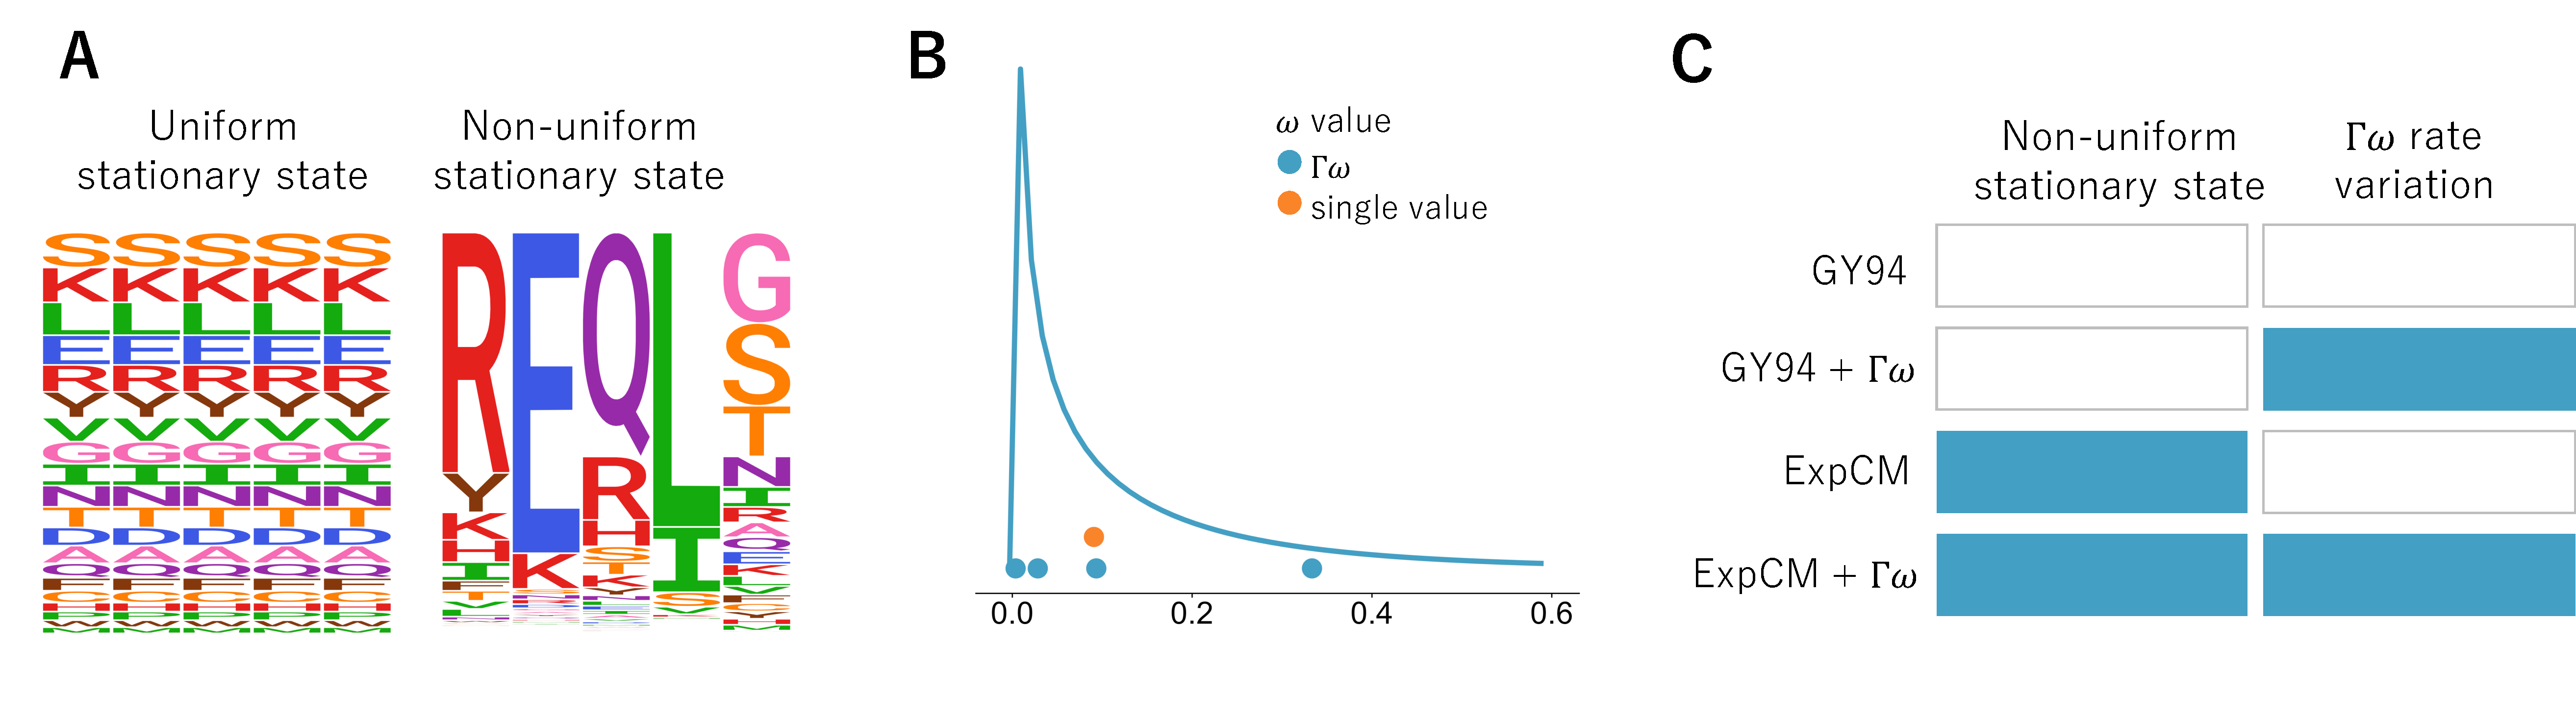
\includegraphics[width=0.90\textwidth]{figures/model_feature.pdf}}
\caption{\label{fig:model_feature}
\textbf{Different ways of modeling the site-to-site rate variation of purifying selection.}
(A) The dN/dS parameter, $\omega$, can be defined as one gene-wide average (orange triangle) or allowed to vary following some statistical distribution (blue circles). 
In order to achieve computational tractability, the distribution is discretized into $K$ bins and $\omega$ takes on the mean of each bin. 
A gamma distribution ($\Gamma$) with $K=4$ bins is shown here.
(B) A substitution model stationary state defines the expected sequence composition after a very long evolutionary time. 
Most substitution models have stationary states that are uniform across sites.
However, substitution models can have site-specific stationary states.
In the logo plots, each column is a site in the protein and the height of each letter is the frequency of that amino acid at stationary state. 
(C) Substitution models can incorporate neither, one, or both of these features.
Here we will use substitution models from the \citet{goldman1994codon} (GY94) and experimentally informed codon model~\citep[ExpCM;][]{hilton2017phydms} families with and without gamma-distributed rates to represent all possible combinations. 
%Green indicates presence of a feature and white indicates absence. 
}
\end{figure}

Proteins evolve under purifying selection to maintain their structure and function. 
This purifying selection is not homogenous across sites in a protein.
It is also not homogenous among the different amino acids at a given site.
For instance, some protein sites strongly prefer hydrophobic amino acids, others may be constrained to just one or a few amino acids, and yet others may tolerate many amino acids.
In general, these constraints are highly idiosyncratic among sites, and so pose a challenge for phylogenetic substitution models.

Here we consider how purifying selection is handled by codon substitution models, which are the most accurate of the three classes (nucleotide, amino acid, and nucleotide) of phylogenetic substitution models in widespread use\jdbcomment{find a citation for this and replace word ``accurate'' with something else if appropriate. Perhaps this one or something cited within \url{https://www.ncbi.nlm.nih.gov/pmc/articles/PMC4620419/}}.
Codon substitution models distinguish between two types of substitutions: synonymous and nonsynonymous.
The relative rate of these substitutions is referred to as dN/dS or $\omega$.
In their simplest form, codon substitution models fit a single $\omega$ that represents the gene-wide average selection on nonsynonymous mutations relative to synonymous ones.
Here we will use such substitution models in the form proposed by \citet{goldman1994codon}.
Using the classification scheme of \citet{yang2000codon}, when these models have a single gene-wide $\omega$ they are called M0.
We will refer to the M0 variant of the \citet{goldman1994codon} model simply as GY94.
The gene-wide $\omega$ is usually $<1$\jdbcomment{add citation, most of the site-specific $\omega$ papers will talk about how gene-wide is not sensitive, so we can cite some of those}, and crudely represents the fact that many amino-acid substitutions are under purifying selection.

A single gene-wide $\omega$ ignores the fact that purifying selection is heterogeneous across sites.
The most common strategy to ameliorate this defect is to allow the rate of nonsynonymous change ($\omega$) to vary among sites following some statistical distribution~\citep{yang1994maximum,yang2000codon}.
For instance, in the M5 variant of the GY94 model~\citep{yang2000codon}, $\omega$ follows a gamma distribution as shown in \ref{fig:model_feature}A.
We will denote this model as GY94+$\Gamma\omega$.
A GY94+$\Gamma\omega$ captures the fact that the rate of nonsynonymous change can vary across sites. 
However, this formulation treats all nonsynonymous substitutions equivalently, since the rate is agnostic to the identity of the specific amino-acid mutation. 

A model formulation that accounts for the fact that purifying selection depends on the specific amino-acid mutation is provided by so-called ``mutation-selection'' models~\citep{halpern1998evolutionary}.
These models by explicitly define a different set of amino-acid preferences at each site in the protein. 
This more mechanistic formulation results in a site-specific stationary state (\ref{fig:model_feature}B). 
These models capture the site-to-site variation in amino-acid composition that is an obvious features of real proteins, and generally better describe actual evolution than models with only rate variation~\citep{lartillot2004bayesian, le2008phylogenetic, rodrigue2010mutation,hilton2017phydms,bloom2014experimentally}.

However, the increased realism of mutation-selection models comes at the cost of an increased number of parameters. 
Codon substitution models with uniform stationary states have only a modest number of parameters that must be fit from the phylogenetic data.
For instance, a GY94 M5 model with the typical F3X4 stationary state\jdbcomment{add citation, maybe just GY94 paper?} has 12 parameters: two describing the shape of the gamma distribution over $\omega$, a transition-transversion rate, and 9 parameters describing nucleotide composition of the stationary state.
However, mutation-selection models must additionally specify 19 parameters defining the stationary state for \emph{each} site (there are 20 amino acids whose frequencies are constrained to sum to one).
This corresponds to $19\times L$ parameters for a protein of length $L$, or 9500 parameters for a 500-residue protein.
It is challenging to obtain values for these parameters without overfitting the data~\citep{rodrigue2013statistical}.
Here we will primarily use experimentally informed codon models (ExpCM)~\citep{bloom2014experimentally, hilton2017phydms, bloom2017identification} which define values for these parameters \textit{a priori} from deep mutational scanning experiments~\citep{fowler2014deep} so they do not need to be fit from phylogenetic data.
Therefore, the number of remaining free parameters for an ExpCM are similar to a non-site-specific substitution model.
Alternative strategies of obtaining parameters for site-specific stationary states via Bayesian\skhcomment{cite} or maximum-likelihood estimation\skhcomment{cite} are discussed in the last section of the Results.

Importantly, these two strategies for modeling purifying selection are not mutually exclusive.
Mutation-selection models such as ExpCM can still incorporate an $\omega$ parameter, which now represents the relative rate of nonsynonymous to synonymous substitution \emph{after} accounting for the constraints due to the site-specific stationary state.
This $\omega$ parameter for an ExpCM can be drawn from a distribution just like for GY94-style models. 
We will denote such models as ExpCM+$\Gamma\omega$.
\ref{fig:model_feature}C shows the full spectrum of models that incorporate all combinations of gamma-distributed $\omega$ and site-specific stationary states.

\subsection*{Effect of stationary state and rate variation on branch-length estimation}

\begin{figure}
\centerline{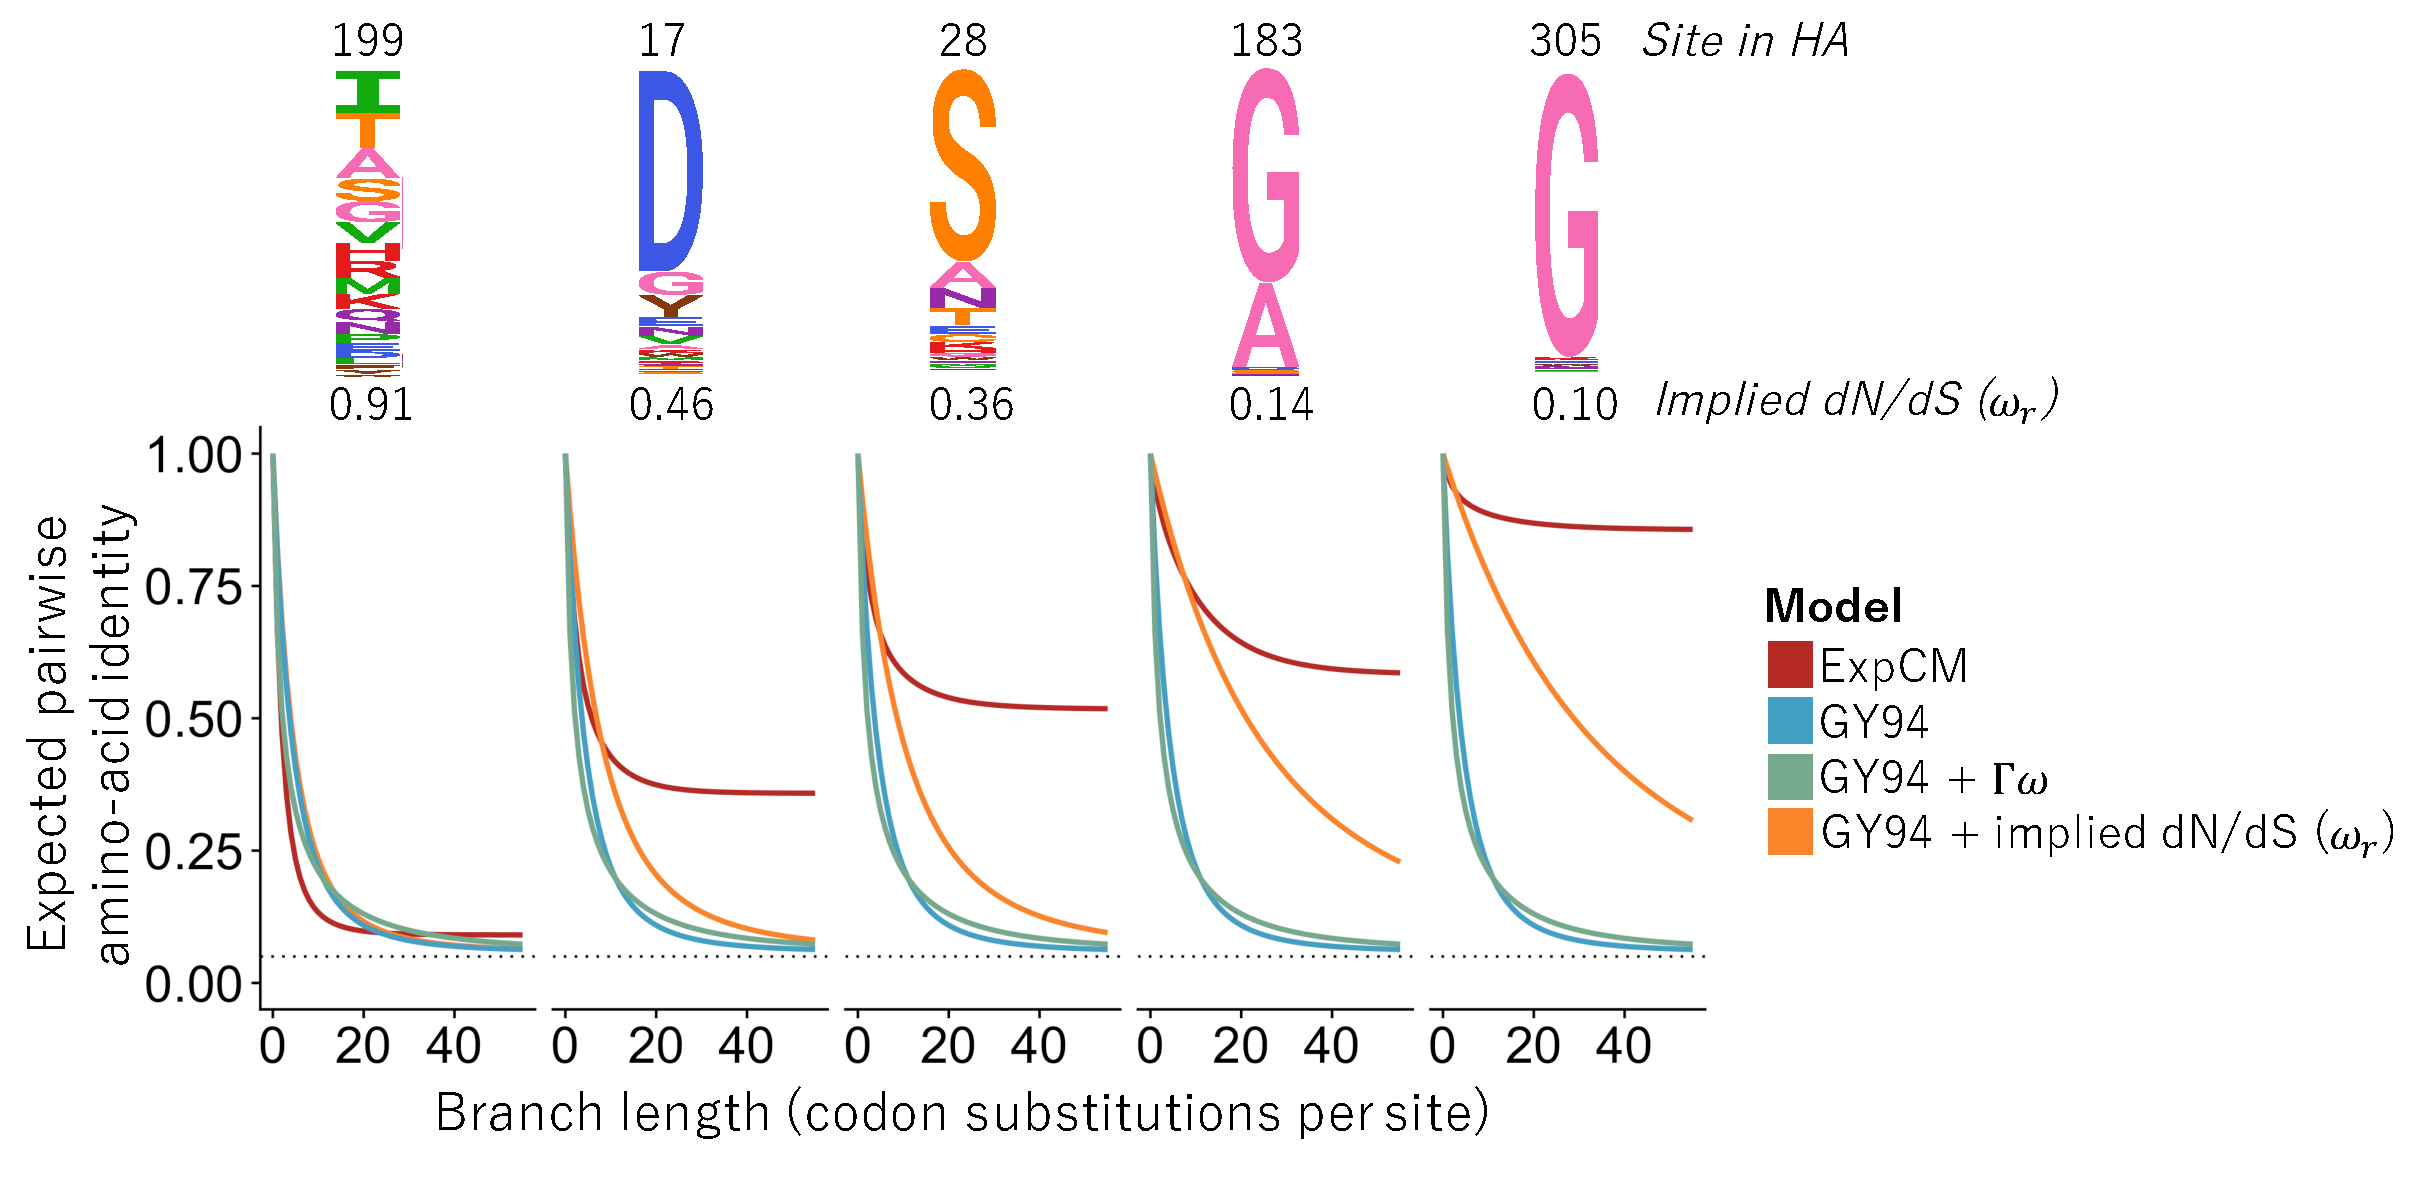
\includegraphics[width=0.90\textwidth]{figures/decay.pdf}}
\caption{\label{fig:decay}
\textbf{Effect of stationary state and $\Gamma\omega$ rate variation on predicted asymptotic sequence divergence.}
The logo plots at top show the amino-acid preferences for some sites in an H1 influenza hemagglutinin protein as measured by \citet{doud2016accurate}.
The graphs show the expected amino-acid identity at that site for two sequences separated by a branch of the indicated length (\ref{eq:f}).
For the GY94 model, the graphs are identical for all sites since this models does not have site-specific parameters; the same is true for GY94+$\Gamma\omega$.
The graphs do differ among sites if we use the amino-acid preferences to calculate a different $\omega_r$ value for each site $r$ in a GY94 framework~\citep[\ref{eq:w_r};][]{spielman2015relationship}.
However, all GY94 models including the one with site-specific $\omega_r$ values all approach the same asymptote since they all have the same stationary state.
But the ExpCM has different asymptotes for different sites since it accounts for how amino-acid preferences lead to site-specific stationary states.
}
\end{figure}

Given a single branch, a substitution model transforms sequence identity into branch length.
Under a molecular-clock assumption, this branch length is proportional to time.
The transformation from sequence identity to branch length is trivial when the sequence identity is high.
For instance, when where there has only been one substitution, then the sequence identity will simply be $\frac{L - 1}{L}$ for a gene of $L$ sites, and even a simple exponential model~\citep{zuckerkandl1965} will correctly infer the short branch length of $1/L$ substitutions per site.
However, as more substitutions accumulate then it becomes progressively more likely for multiple changes to occur at the same site.
In this regime, the accuracy of the substitution model becomes critical for transforming the sequence identity into branch length.
Any time-homogenous substitution model predicts that after a very large number of substitutions, two related sequences will approach some asymptotic sequence identity.
For instance, if all 20 amino acids are equally likely in the stationary state, then this asymptotic sequence identity will be 0.05.
If the substitution model underestimates the asymptotic sequence divergence then it will also underestimate long branch lengths, since it will predict that long branches lead to more divergence lead than is actually the case.

\ref{fig:decay} shows how different substitution models predict sequence identity to decrease as a function of branch length for model parameters fit to a phylogeny of H1 influenza hemagglutinin (HA) genes.
The GY94 predicts the same behavior for all sites, since it does not have any site-specific parameters.
This model predicts an asymptotic sequence divergence of \jdbcomment{?}, which is slightly higher than 0.05 since some of the 20 amino acids are favored due to more redundant codons and biases towards certain nucleotides.
Intuitively, this asymptotic sequence identity of \jdbcomment{?} seems low, since like many proteins HA has a highly conserved structure and function which imposes constraints that cause some sites to only sample a small subset of the 20 amino acids among all known HA homologs.

Accounting for site-to-site rate variation in GY94 models affects the rate at which the asymptotic sequence identity is approached, but not the actual value of this asymptote. 
For instance, \ref{fig:decay} shows that the GY94+$\Gamma\omega$ model takes longer to reach the asymptote than GY94, but the asymptote for both models is identical. 
This fact holds true even if we use experimental measurements of HA's site-specific amino-acid preferences~\citep{doud2016accurate} to calculate a different $\omega_r$ value for each site using the method of \citet[\ref{eq:w_r};][]{spielman2015relationship}.
Specifically, this GY94+$\omega_r$ model predicts that different sites will approach the asymptote at different rates, but the asymptote is always the same (\ref{fig:decay}).
The invariance of the asymptotic sequence identity under different schemes for modeling $\omega$ is a fundamental feature of the mathematics of homogeneous substitution models.
The asymptotic sequence divergence is a function of only the stationary state of the substitution matrix, and the stationary state of a stochastic matrix is invariant with respect to multiplication by any non-zero number\jdbcomment{But this isn't true, because $\omega$ only multiplies some elements of transition matrix. I think it's probably something like if you multiple pairs of elements on equivalent positions across diagonal?}.
Therefore, different schemes for modeling $\omega$ can alter the time it takes to reach stationary state, but no matter how ``well" a model accounts for site-to-site variation in $\omega$ it will always have the same stationary state as a simple GY94 model. 

\jdbcomment{In contrast, ExpCM models have different stationary states at each site...}

We visualized the effect of stationary state on branch length estimation by examining the expected amino-acid identity of a set of sequences given some branch length for site-specific and uniform stationary state models. 
By definition, the expected identity given a very long time varies from site to site for the site-specific stationary state models (\ref{fig:decay}, ExpCM, red) but is constant across sites for the uniform stationary state models (\ref{fig:decay}, GY94, blue). 
Due to the assumed equivalence of amino-acid preferences in the GY94 model, the biggest difference in stationary state between the ExpCM and the GY94 is seen at constrained sites, such as site 305 in \ref{fig:decay}. 
The ExpCM would estimate a much longer branch than the GY94 model given some observed divergence at such a site. 



However, a complicating factor in this estimation procedure is the stationary state of the model. 
Stationary state, as the principle eigenvector of a stochastic matrix, is a fundamental feature of any substitution model. 
It describes the expected sequence composition after a very long evolutionary time. 
Additionally, the stationary state does not change under application of the transition matrix, which means this sequence composition remains constant as time increases. 
The invariance of the stationary state is represented by the long ``tails" in \ref{fig:decay}. 
The exact sequence composition of stationary state is unique given the parametrization of the model. 

\subsection*{Failure to account for site-specificity leads to branch length underestimation.}

\begin{figure}[H]
\centerline{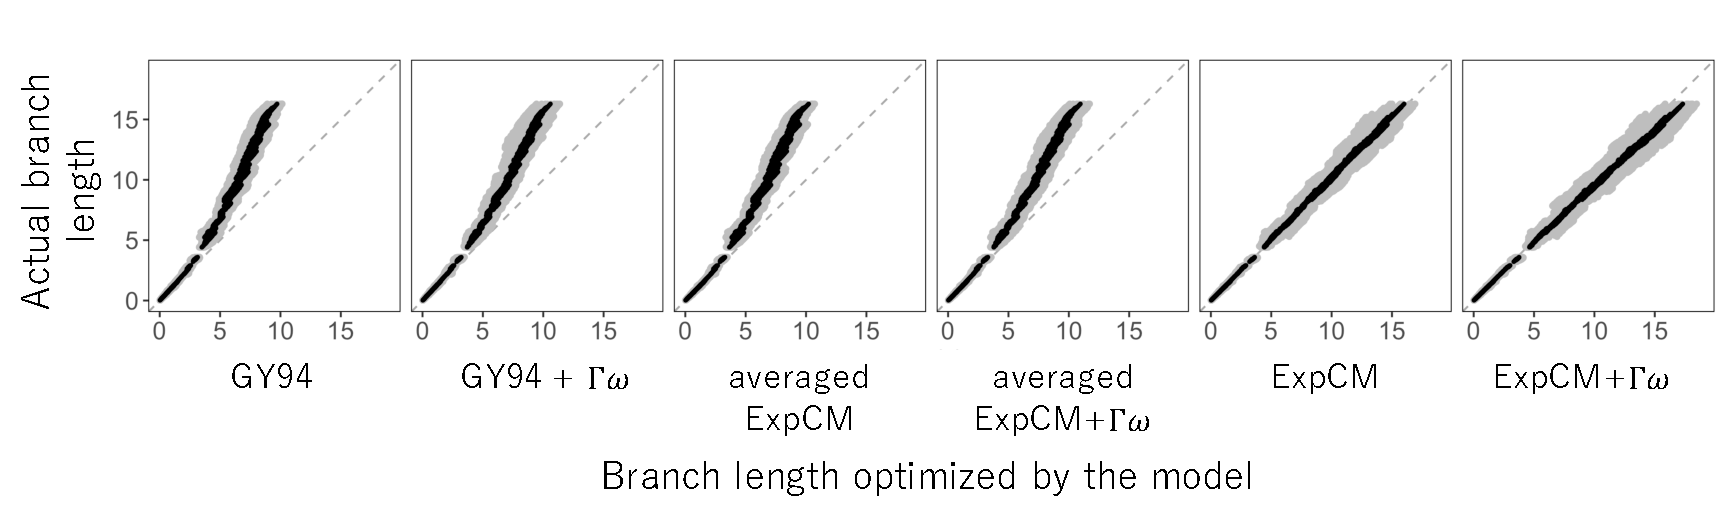
\includegraphics[width=0.85\textwidth]{figures/simulations}}
\caption{\label{fig:simulations}
\textbf{Model performance under simulated, site-specific data.} 
Alignments were simulated under an ExpCM and branch lengths were re-estimated using models from the ExpCM and GY94 families. 
The averaged ExpCMs have a uniform stationary state defined by the average preference for each amino acid across all sites in the protein. 
The length of one branch in one simulation is shown in grey and the average length of one branch across ten simulations is shown in black. 
The grey, dashed reference line $y=x$ represents the behavior of an unbiased estimator. 
}
\end{figure}

Next, we tested the effect of stationary state and $\Gamma\omega$ rate variation on branch length estimation given sequences with site-specific amino-acid frequencies. 
We simulated sequences under an ExpCM, re-estimated the branch lengths using the models in \ref{fig:model_feature}C, and compared these estimates to the actual branch lengths.

The models with a uniform stationary state underestimated the branch lengths of the simulated sequences, especially the lengths of long branches. 
The GY94 model estimated branches lengths which are only about 60\% of the true branch length for the longest branches. 
Accounting for site-to-site rate variation by $\Gamma\omega$ did not prevent the underestimation of long branches, as the GY94+$\Gamma\omega$ inferred approximately the same branch lengths as the GY94 model.
We also estimated branch lengths using averaged ExpCMs.
The averaged ExpCMs have a uniform stationary state defined by the average DMS preference for a given amino acid across all sites from the deep mutational scan. 
Even these models, which share information with the model used to simulate the sequences, underestimated the long branches. 
The inability of these uniform stationary state models to specifically describe purifying selection on a site by site basis clearly hinder their ability to accurately estimate long branch lengths. 

Neither the ExpCM nor the ExpCM+$\Gamma\omega$ underestimated the long branches. 
This is an unsurprising result, as the sequences were simulated under an ExpCM. 
However, while not biased towards over- or underestimation, the variance between simulations increased as the branch length increased. 
The increase in error, even with a perfect model match, underscores the difficulty of estimating extremely long branches. 
Despite this universal difficulty, it is clear from the GY94 and averaged ExpCM results that models with a uniform stationary state will always drastically underestimate long branches. 

\subsection*{empirical Data}

\begin{figure}[H]
\centerline{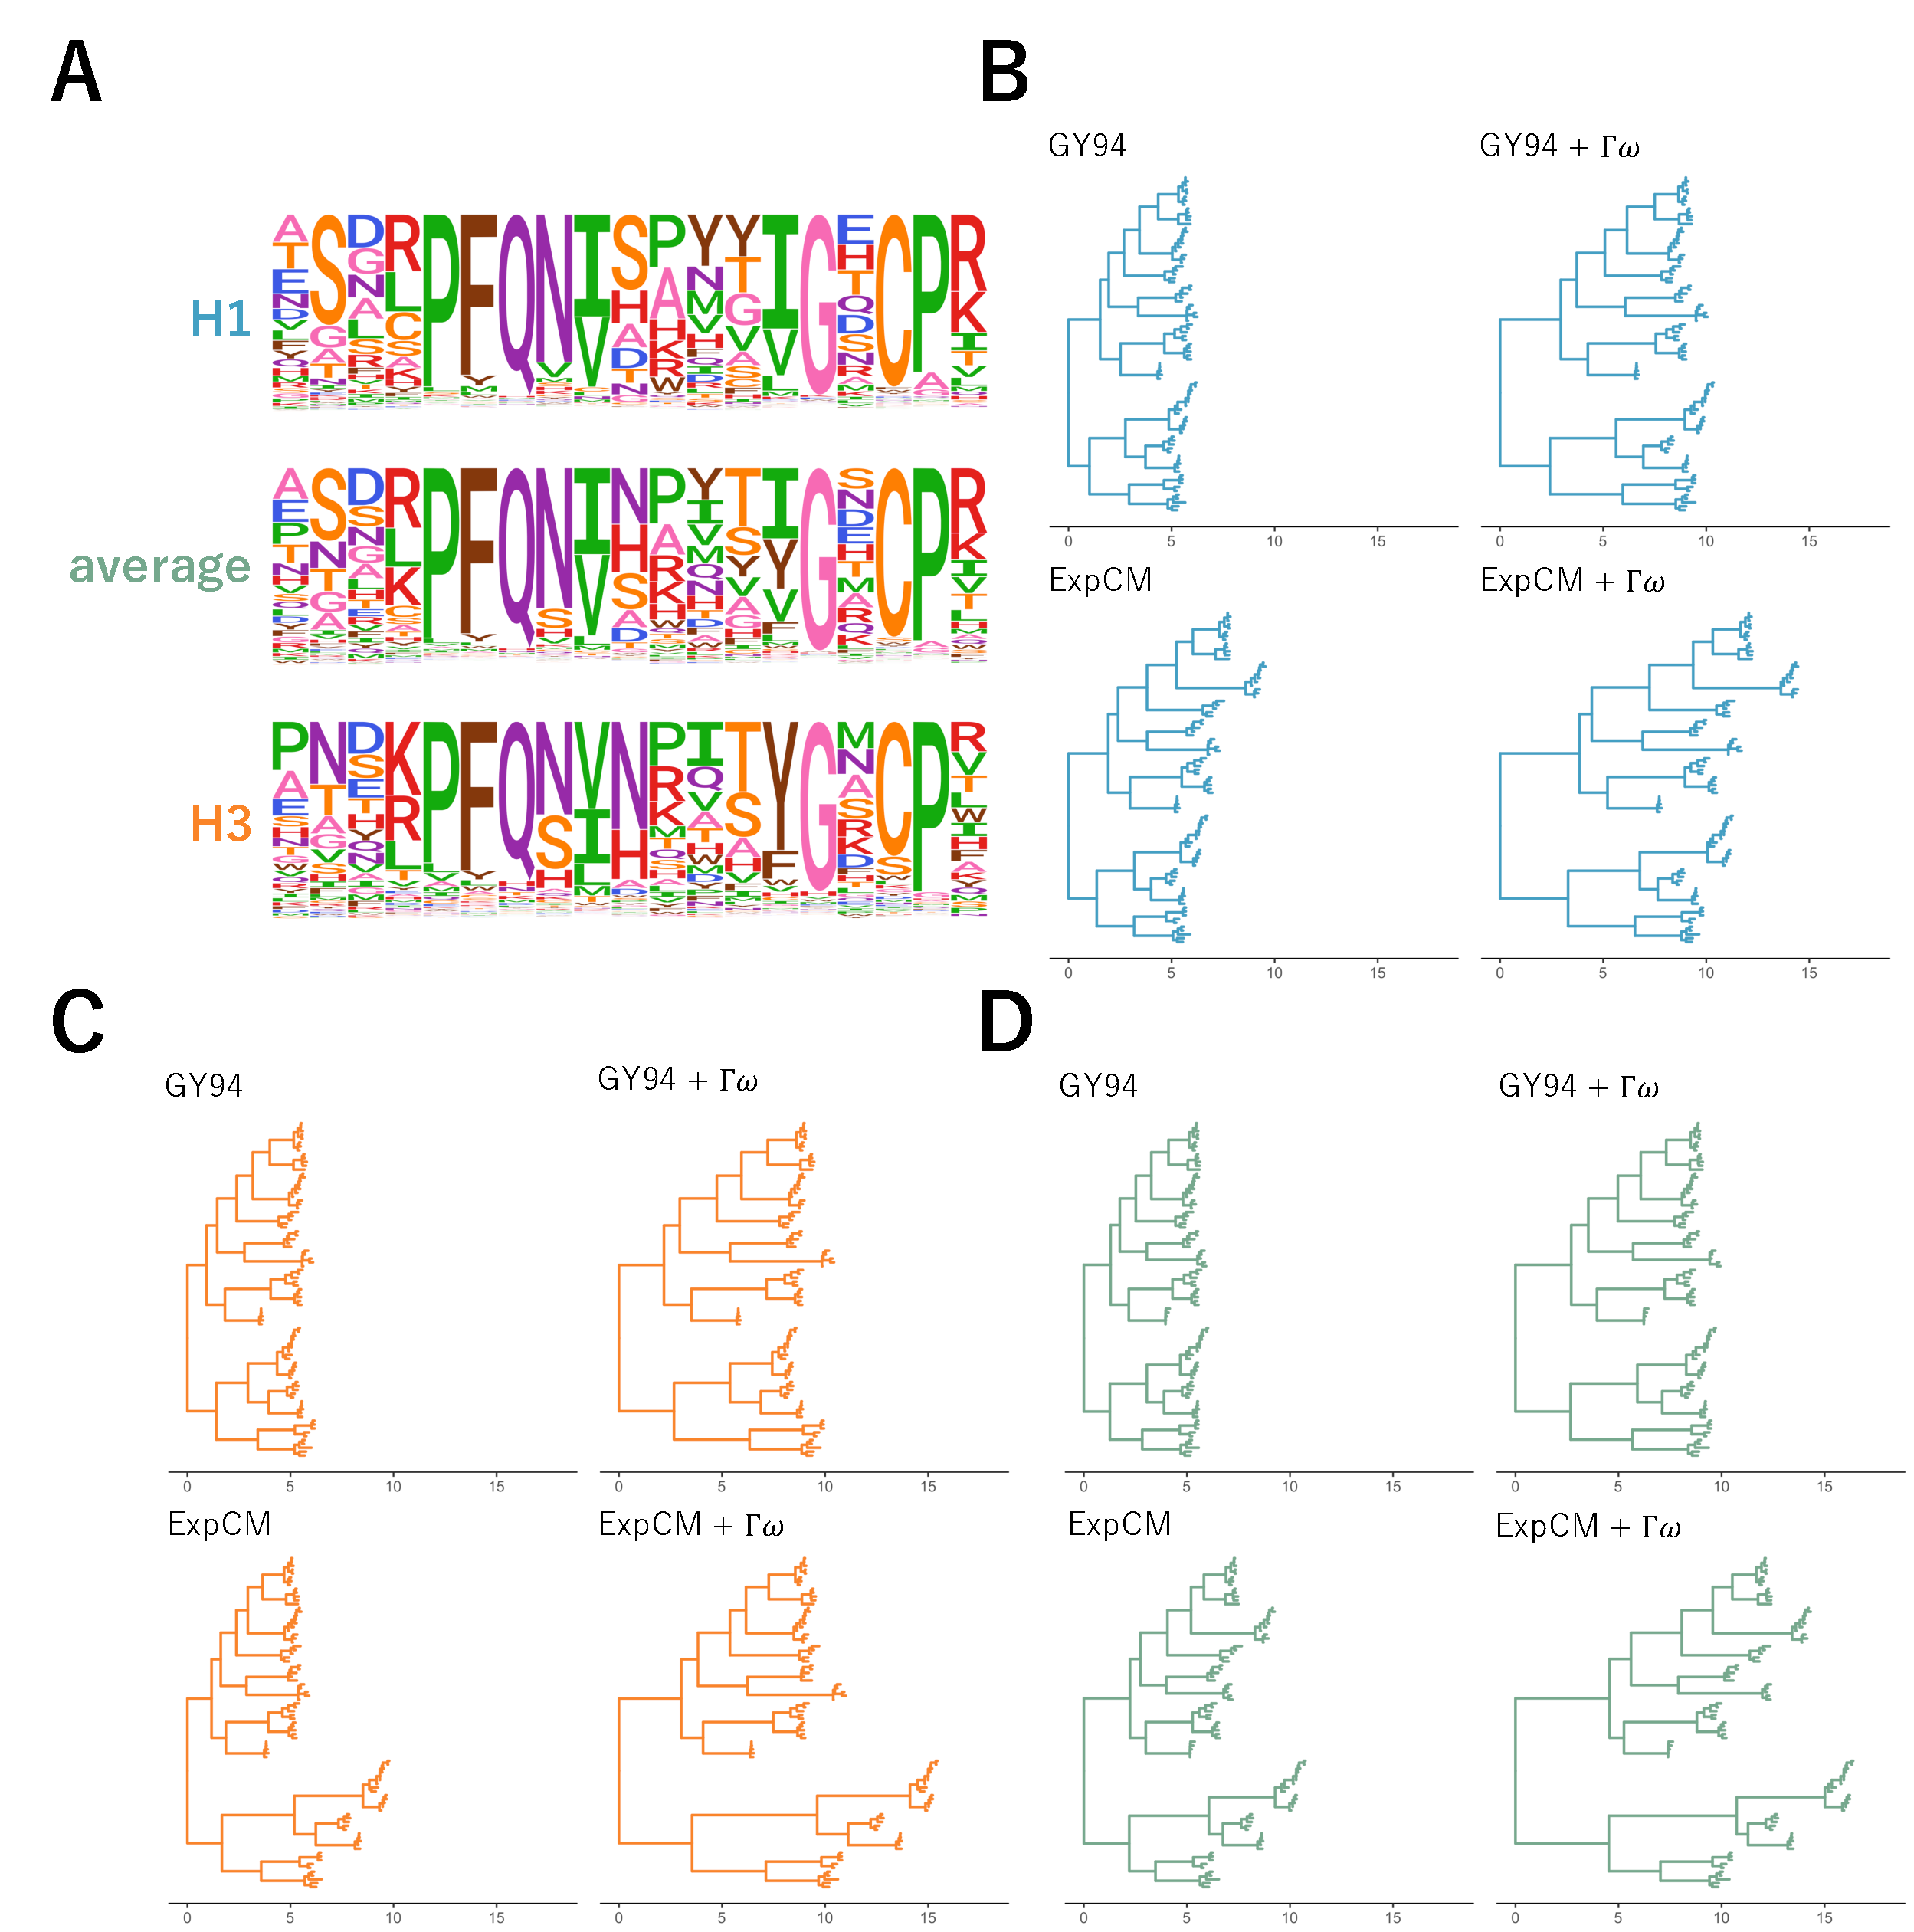
\includegraphics[width=0.8\textwidth]{figures/empirical_trees.pdf}}
\caption{\label{fig:empirical_trees}
\textbf{Effect of site-specific stationary state and $\Gamma\omega$ rate variation on HA branch length estimation.} 
The HA tree is optimized by models from the ExpCM and GY94 families. 
The amino-acid preferences defining the model (ExpCM) or implied by the model (GY94) are shown as logoplots. 
The amino-acid preferences measured by the deep mutational scans defining the ExpCMs were measured in either an H1 background, an H3 background, or were the average measurements from the H1 and H3 scans. 
The circle denotes the H1 clade and the triangle denotes the H3 clade. 
}
\end{figure}

\begin{table}[t!]
\caption{\label{tab:empirical_data}
Performance comparison for the models in~\ref{fig:empirical_trees}. 
All ExpCMs describe the evolution of HA better than the GY94 models, as evaluated by the Akaike information criteria~\citep[$\Delta$AIC,][]{posada2004model}
The mean $\omega$ value from each $K=4$ bins is shown for the models with $\Gamma\omega$ rate variation, otherwise simply the fit, gene-wide $\omega$. 
Each ExpCM has a stringency parameter $>1$.
\skhcomment{GY94+$\Gamma\omega$ has one $\omega$ of 0 because of rounding.}
} 
     \begin{tabular}{cccccccccc}
        \hline
         Model & {\shortstack{Site-specific\\ stationary state}} & $\Gamma\omega$ & $\Delta$AIC & {\shortstack{Log\\ Likelihood}} & {\shortstack{$\omega$\\ (implied dN/dS)}} & {\shortstack{stringency\\ parameter}}\\ \hline
       	ExpCM + $\Gamma\omega$ (H1+H3 avg) & + & + & 0 & -487510 & 0.19,  0.50,  0.90,  1.86 &  1.70\\
	ExpCM (H1+H3 avg) & + & - &  950 & -492270 & 0.15 & 1.78\\
	ExpCM + $\Gamma\omega$ (H1) & + & + & 1306 & -494040  & 0.13 ,  0.44,  0.91,  2.16 & 1.12\\
	ExpCM + $\Gamma\omega$ (H3) & + & + & 1737 & -49620 & 0.09,  0.33,  0.72,  1.77 & 1.28\\
	ExpCM (H1) & + & - & 2556 & -50030 &  0.13 & 1.22\\
	ExpCM (H3) & + & - &  3197 & -50350 & 0.12 & 1.45\\
	GY94 + $\Gamma\omega$ & - & + & 4719 & -51106 & 0.00,  0.03,  0.08,  0.26 & - \\
	GY94 & - & - & 7625 & -52560  & 0.07 & -\\
      \end{tabular}
\end{table}

Next, we wanted to examine the effect of substitution model on branch length estimation for actual protein coding sequences. 
We assume protein coding sequences have site-specific amino-acid preferences, but unlike the simulations, we do not know the underlying model.
We used sequences from the influenza virus surface protein hemagglutinin (HA). 
The HA tree structure makes it a useful model for studying long branch estimation; HA is conserved within any given subtype but the subtypes themselves are separated by long branches. 
The most diverged subtypes on the HA tree are only about 40\% identical on the amino acid level. 
We used an HA tree with 87 sequences from 14 of the 18 subtypes, excluding subtypes with very few sequences. 

We estimated the branch lengths on this HA tree using the models in \ref{fig:model_feature}C. 
We used two different ExpCMs defined by different deep mutational scanning experiments from different HA homologs. 
One scan measured the site-specific amino-acid preferences in an H1 background (\ref{fig:empirical_trees}, circle) and the other measured the preferences in an H3 background (\ref{fig:empirical_trees}, triangle). 
These two deep mutational scans sample the breadth of HA diversity as their respective focal sequences are only $\sim42\%$ identical on the amino acid level. 
By comparing these two ExpCMs, we can examine the effect of the experiment's focal sequence on branch length estimation, along with the effect of site-specific stationary state and $\Gamma\omega$ rate variation.

Models with either site-specific stationary state or $\Gamma\omega$ rate variation estimated longer branches than models without (\ref{fig:empirical_trees}). 
Furthermore, we can isolate the effect of each method. 
For example, the increase in branch length estimated by GY94+$\Gamma\omega$ compared to GY94 and by ExpCM+$\Gamma\omega$ compared to ExpCM shows that $\Gamma\omega$ rate variation increases branch length in the presence and absence of a site-specific stationary state. 
We also see an increase in branch length with the addition of a site-specific stationary state in the presence and absence of $\Gamma\omega$ rate variation (\ref{fig:empirical_trees}, GY94 vs. ExpCM and GY94+$\Gamma\omega$ vs. ExpCM+$\Gamma\omega$). 
The model with both methods, ExpCM+$\Gamma\omega$, estimated the longest branches of all the models. 
However, the branch length extension from any of the ExpCM compared to any of the GY94 models was not uniform across the entire tree. 
The branches with the largest difference in branch length are near the focal sequence of the deep mutational scans (\ref{fig:empirical_trees}, circle for H1 and triangle for H3)
This local effect of the ExpCM indicates that the stationary state described by the deep mutational scanning preferences is most accurate near the focal sequences of the scan. 

The local effect of the ExpCM is not entirely surprising. 
Proteins are affected by epistatic interactions, where the effect of a mutation at one site is dependent on the amino-acid identity at another site. 
While one of the strengths of deep mutational scanning is the ability to accurately measure the effect of all single amino-acid mutations, these measurements are done in the context of a single genetic background and do not take into account epistatic interactions. 
Consequently, the stationary state defined by these preferences is most accurate for only a subset of the tree.
An ExpCM with a more general stationary state, defined by the average of the H1 and H3 preferences, lengthen the preferences from both the H1 and H3 clades (\ref{fig:empirical_trees}). 

\subsection*{Competing effects of shifting preferences and long branches.}

\begin{figure}[H]
\centerline{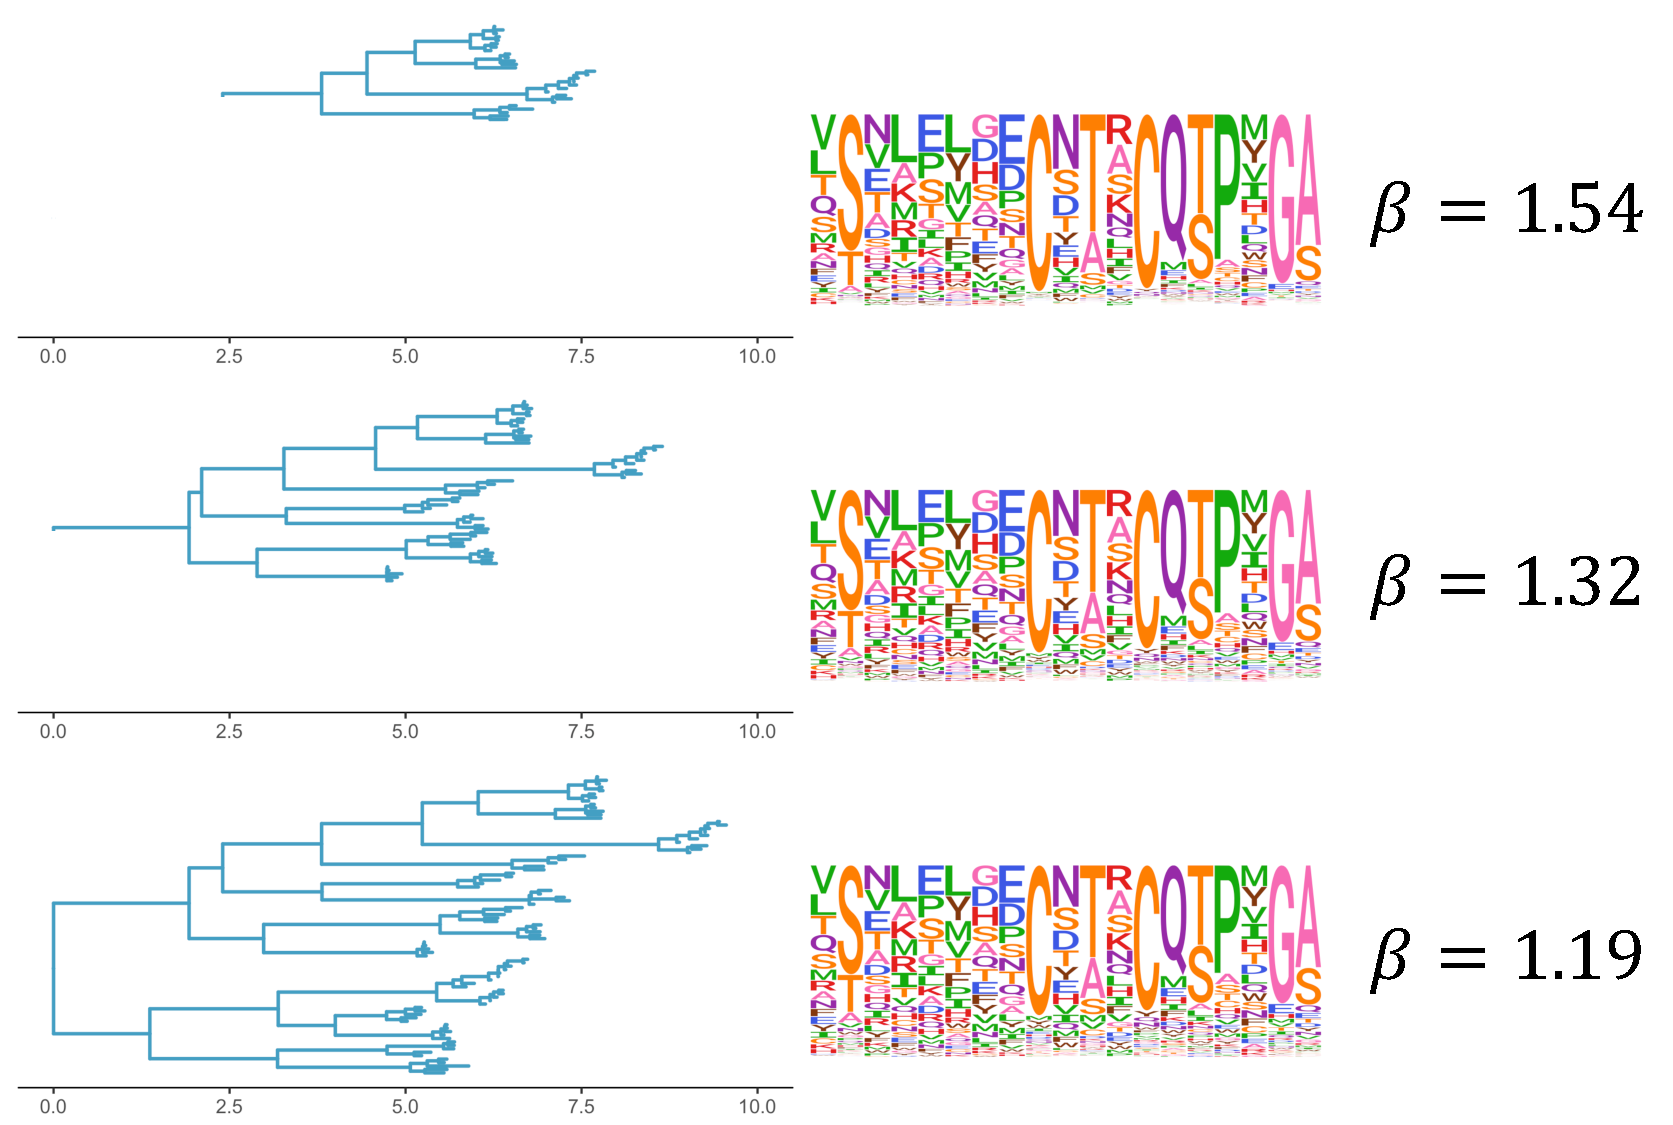
\includegraphics[width=0.85\textwidth]{figures/doud_compete_2}}
\caption{\label{fig:doud_compete}
\textbf{The ExpCM defined by H1 preferences lengthen longer branches on the HA tree.} 
\textbf{(A)} An HA alignment was subsampled to create three smaller alignments with varying degrees of divergence from the focal H3 sequence, referred to as "low", "intermediate", and "high". 
\textbf{(B)} The phylogenetic tree of the "high" alignment. 
The colors denote the alignment and the black circle denotes the focal H3 sequence. 
\textbf{(C)} The value of the ExpCM and ExpCM+$\Gamma\omega$ stringency parameter $\beta$ decreases as the divergence from the focal H3 sequence increases. 
\textbf{(D)} Comparisons of branch lengths optimized by the four substitution models for the varying degrees of divergence. 
Black points represent branches from the focal H3 sequence and grey points represent all other branches.  
The branch lengths are in average number of codon substitutions per site. 
}
\end{figure}

We looked closer at the effect of shifting preferences on branch length estimation. 
We examined the behavior of the ExpCM on trees with varying levels of overall sequence divergence from the ExpCM focal sequence. 
For each tree, we asked ``does the site-specific stationary state model estimate longer branches than the uniform stationary state model?" and ``is the preference set defining the ExpCM relevant?"

The effect of site-specific stationary state on branch length estimation is seen most strongly on long branches. 
As the full HA tree represents ``high" divergence from the DMS focal sequence, we took subsets the tree to create trees with either ``intermediate" or ``low" divergence from the DMS focal sequence. 
The majority of the branch length estimates are very similar between the GY94+$\Gamma\omega$ and the ExpCM+$\Gamma\omega$ for the ``low" and ``intermediate" alignments. 
Only when the tree has a high overall divergence from the DMS focal sequence, and therefore the longest branches, is there a difference between the two models. 
This result is not unsurprising. 
One of the original motivations for the ``mutation-selection" models was the effect the model would have on long branches specifically. 

We wanted to determine the accuracy or relevance of the ExpCM on these subtrees. 
Due to the local branch length extension in \ref{fig:empirical_trees}, we expect that the preferences are most accurate on the low divergence tree. We use the ExpCM stringency parameters as a proxy for accuracy of the preference set. 
The stringency parameter rescales the raw preferences from the deep mutational scan. 
Large stringency parameter values ($>1$) indicate that selection in nature prefers the same amino acids as selection in lab but with a higher stringency.
Or that the preferences measured in lab are relevant for describing the evolution of that protein. 
The stringency parameter for ExpCM(H1 prefs) has the highest value for the low divergence alignment and declines as the overall divergence increases. 
The ExpCM(H3 prefs) show the same pattern. 
The inverse relationship between stringency parameter and divergence supports the hypothesis that epistatic interactions degrade the ExpCM stationary state as defined by DMS preferences. 
\skhcomment{All epistatic? Could there just be a change?}

Current models which have one stationary state across the entire tree, site-specific or not, will not be able to address this tension. 

\subsection*{\texttt{phylobayes}}

Finally, we compared the branch lengths estimated between two different models with site-specific stationary states. 
We compared the branch lengths estimated by ExpCM+$\Gamma\omega$ (avg) with the branch lengths estimated by the mutation-selection model implemented in \texttt{phylobayes}. 
The \texttt{phylobayes} mutation-selection model estimates the amino-acid preferences which define the stationary state in a Bayesian framework rather than defining them from the DMS \textit{a priori}. 
Branch length estimates are very similar between the ExpCM+$\Gamma\omega$ (avg) and the \texttt{phylobayes} mutation-selection model. 
The equivalence between the two models shows the general importance of site-specific stationary states. 
The local accuracy of the DMS preferences and the ExpCM can still be seen. 
The branch length estimates from either focal sequence (H1 and H3) are longer by the ExpCM than by the \texttt{phylobayes} mutation-selection model. 
This indicates that the DMS preferences are still more accurate for the local branches around the focal sequence than the global preferences estimated by \texttt{phylobayes}. 

\skhcomment{What is the average difference in branch length between the two models?}

\begin{figure}[H]
\centerline{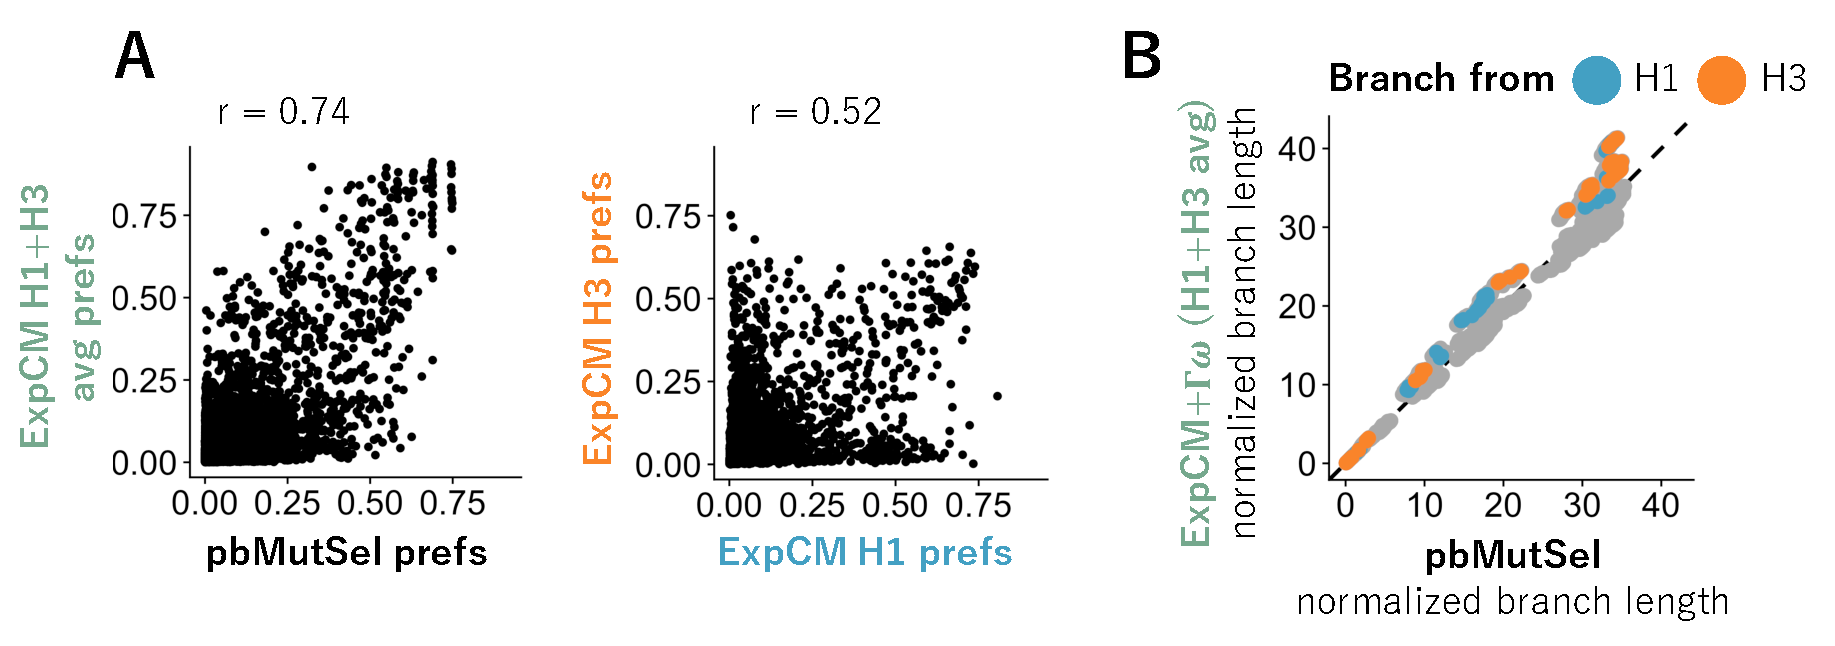
\includegraphics[width=0.5\textwidth]{figures/phylobayes.pdf}}
\caption{\label{fig:phylobayes}
\textbf{Comparison of ExpCM and phylobayes}
\skhcomment{y=x line too faint?}
}
\end{figure}

\section*{Conclusion}

\begin{enumerate}
  \item We don't allow any of the models to vary by lineage. 
\end{enumerate}

\newpage
\section*{Materials and Methods}

\subsection*{Substitution models}
\subsubsection*{GY94 models}
\subsubsection*{ExpCMs}
We recap the \textbf{Exp}erimentally Informed \textbf{C}odon \textbf{M}odel (ExpCM) \citep{bloom2014experimentally,bloom2014informed,bloom2017identification,hilton2017phydms} to introduce nomenclature. 

In an ExpCM, rate of substitution $P_{r,xy}$ of site $r$ from codon $x$ to $y$ is written in mutation-selection form~\citep{halpern1998evolutionary,mccandlish2014modeling,spielman2015relationship} as
\begin{equation}
P_{r,xy} = Q_{xy} \times F_{r,xy}
\end{equation}
where $Q_{xy}$ is proportional to the rate of mutation from $x$ to $y$, and $F_{r,xy}$ is proportional to the probability that this mutation fixes.
The rate of mutation $Q_{xy}$ is assumed to be uniform across sites, and takes an HKY85-like~\citep{hasegawa1985dating} form:
\begin{equation}
Q_{xy} = 
\begin{cases}
\phi_w & \mbox{if $x$ and $y$ differ by a transversion to nucleotide $w$} \\
\kappa \phi_w & \mbox{if $x$ and $y$ differ by a transition to nucleotide $w$} \\
0 & \mbox{if $x$ and $y$ differ by $>1$ nucleotide.}
\end{cases}
\end{equation}
The $\kappa$ parameter represents the transition-transversion ratio, and the $\phi_w$ values give the expected frequency of nucleotide $w$ in the absence of selection on amino-acid substitutions, and are constrained by $1 = \sum_w \phi_w$.

The deep mutational scanning data are incorporated into the ExpCM via the $F_{r,xy}$ terms.
The experiments measure the preference $\pi_{r,a}$ of every site $r$ for every amino-acid $a$.
The $F_{r,xy}$ terms are defined in terms of these experimentally measured amino-acid preferences as
\begin{equation}
\label{eq:Frxy}
F_{r,xy} = 
\begin{cases}
   1 & \mbox{if $\mathcal{A}\left(x\right) = \mathcal{A}\left(y\right)$} \\
   \omega \times \frac{\ln\left[\left(\pi_{r,\mathcal{A}\left(y\right)} / \pi_{r,\mathcal{A}\left(x\right)}\right)^{\beta}\right]}{1 - \left(\pi_{r,\mathcal{A}\left(x\right)} / \pi_{r,\mathcal{A}\left(y\right)}\right)^{\beta}} & \mbox{if $\mathcal{A}\left(x\right) \ne \mathcal{A}\left(y\right)$}
   \end{cases}
\end{equation}
where $\mathcal{A}\left(x\right)$ is the amino-acid encoded by codon $x$, $\beta$ is the stringency parameter, and $\omega$ is the relative rate of nonsynonymous to synonymous substitutions after accounting for the amino-acid preferences.
The ExpCM has six free parameters (three $\phi_w$ values, $\kappa$, $\beta$, and $\omega$).
The preferences $\pi_{r,a}$ are \emph{not} free parameters since they are determined by an experiment independent of the sequence alignment being analyzed.

The ExpCM stationary state frequency $p_{r,x}$ of codon $x$ at site $r$ is~\citep{bloom2017identification} 
\begin{equation}
\label{eq:p_rx}
p_{r,x} = \frac{\left(\pi_{r,\mathcal{A}\left(x\right)}\right)^{\beta} \phi_{x_0} \phi_{x_1} \phi_{x_2}}{\sum_z \left(\pi_{r,\mathcal{A}\left(z\right)}\right)^{\beta} \phi_{z_0} \phi_{z_1} \phi_{z_2}},
\end{equation}
\subsection*{Theoretical effect of model choice on branch length}
\subsection*{Effect of model choice on natural sequences}

\subsubsection*{ExpCM + $\Gamma\omega$ and YNGKP M5}


\subsubsection*{Spielman $\omega_{r}$ values inferred from the ExpCM} 
We inferred the average nonsynonymous fixation rate from the ExpCM following~\citet{spielman2015relationship} as 
\begin{equation}
\label{eq:w_r}
\omega_{r} = \frac{\sum_{x} \sum_{y \in N_x} {p_{r,x} \times P_{r,xy}}}{\sum_{x} \sum_{y \in N_x} {p_{r,x} \times Q_{xy}}}
\end{equation}
where $p_{r,x}$ is the stationary state of the ExpCM at site $r$ and codon $x$, $P_{r,xy}$ is the substitution rate from codon $x$ to codon $y$ at site $r$, $Q_{xy}$ is the mutation rate from codon $x$ to codon $y$, and $N_x$ is the set of codons that are nonsynonymous to codon $x$ and differ from codon $x$ by only one nucleotide. 

\subsubsection*{Expected pairwise amino-acid identity}
\textit{Do I need to talk about the branchScale scaling I used?}
The expected pairwise amino-acid identity at a site $r$ over time $t$ for a given model is 
\begin{equation}
\label{eq:f}
\sum_a \sum_{x \in a} p_{r,x} \sum_{y \in a} [M_{r}\left(t\right)]_{xy}
\end{equation}
where $a$ is all amino acids, $p_{r,x}$ is the stationary state of the model at site $r$ and codon $x$, and $[M_{r}\left(t\right)]_{xy}$ is the transition rate from codon $x$ to codon $y$ at site $r$ given time $t$. 

\newpage
\section*{Supplemental Information}

\subsection*{Model Parameters for the simulations}

\begin{suppfig}[H]
\centerline{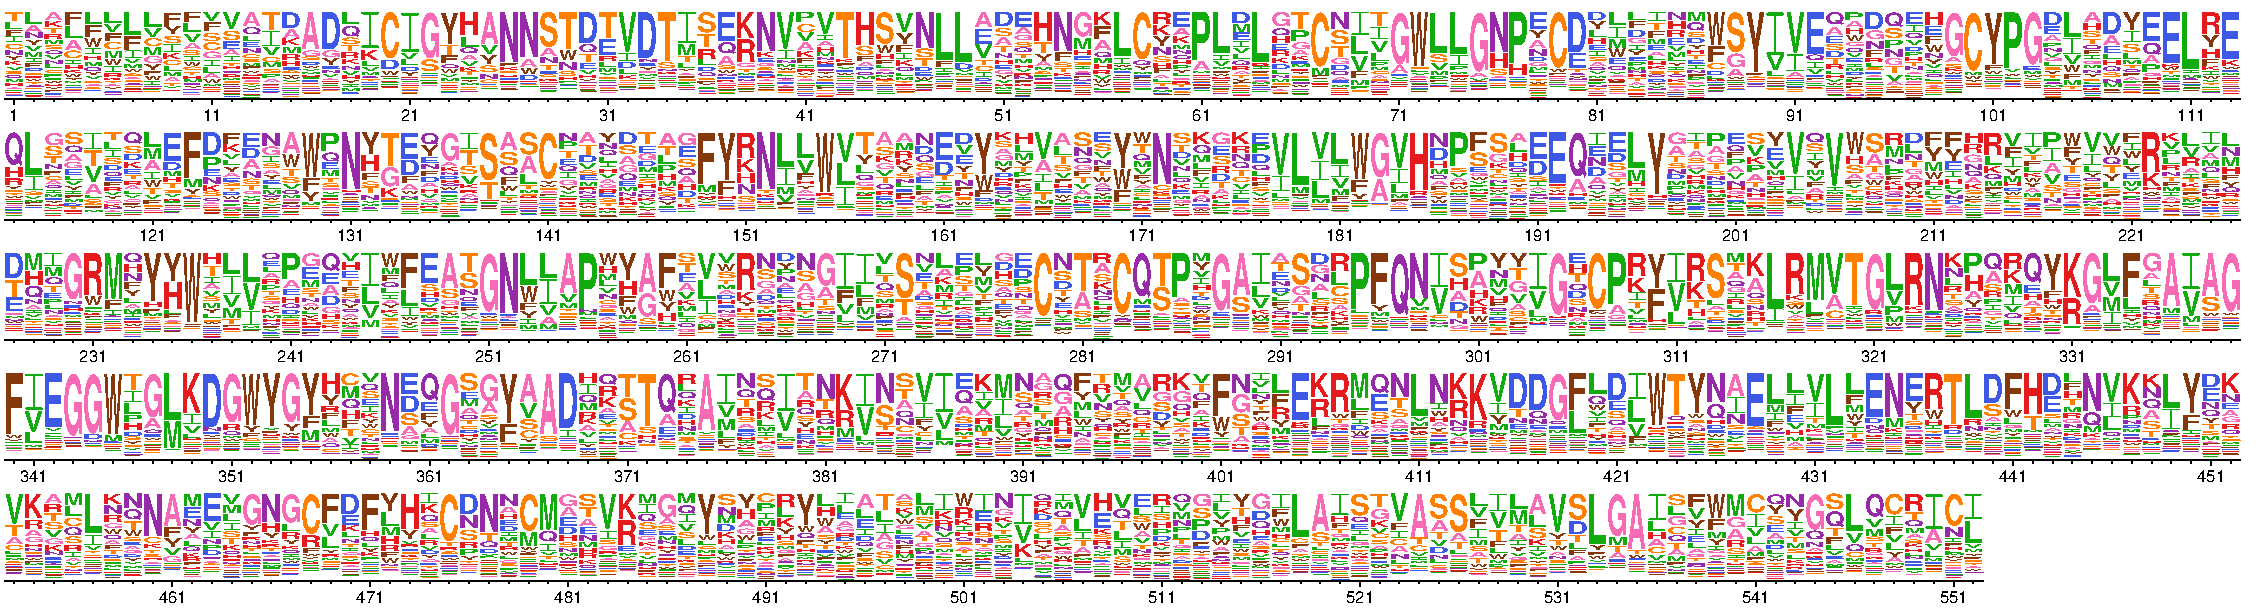
\includegraphics[width=\textwidth]{figures/prefs_doud}}
\caption{\label{suppfig:prefs_doud}
\textbf{H1 preferences measured by \cite{doud2016accurate} rescaled with the ExpCM stringency parameter optimized in \ref{fig:tree_doud}A  ($\beta = 1.19$)} 
\skhcomment{I need to change the $\beta$ value when the new \texttt{phydms} results finish running.}
}
\end{suppfig}

\begin{suppfig}[H]
\centerline{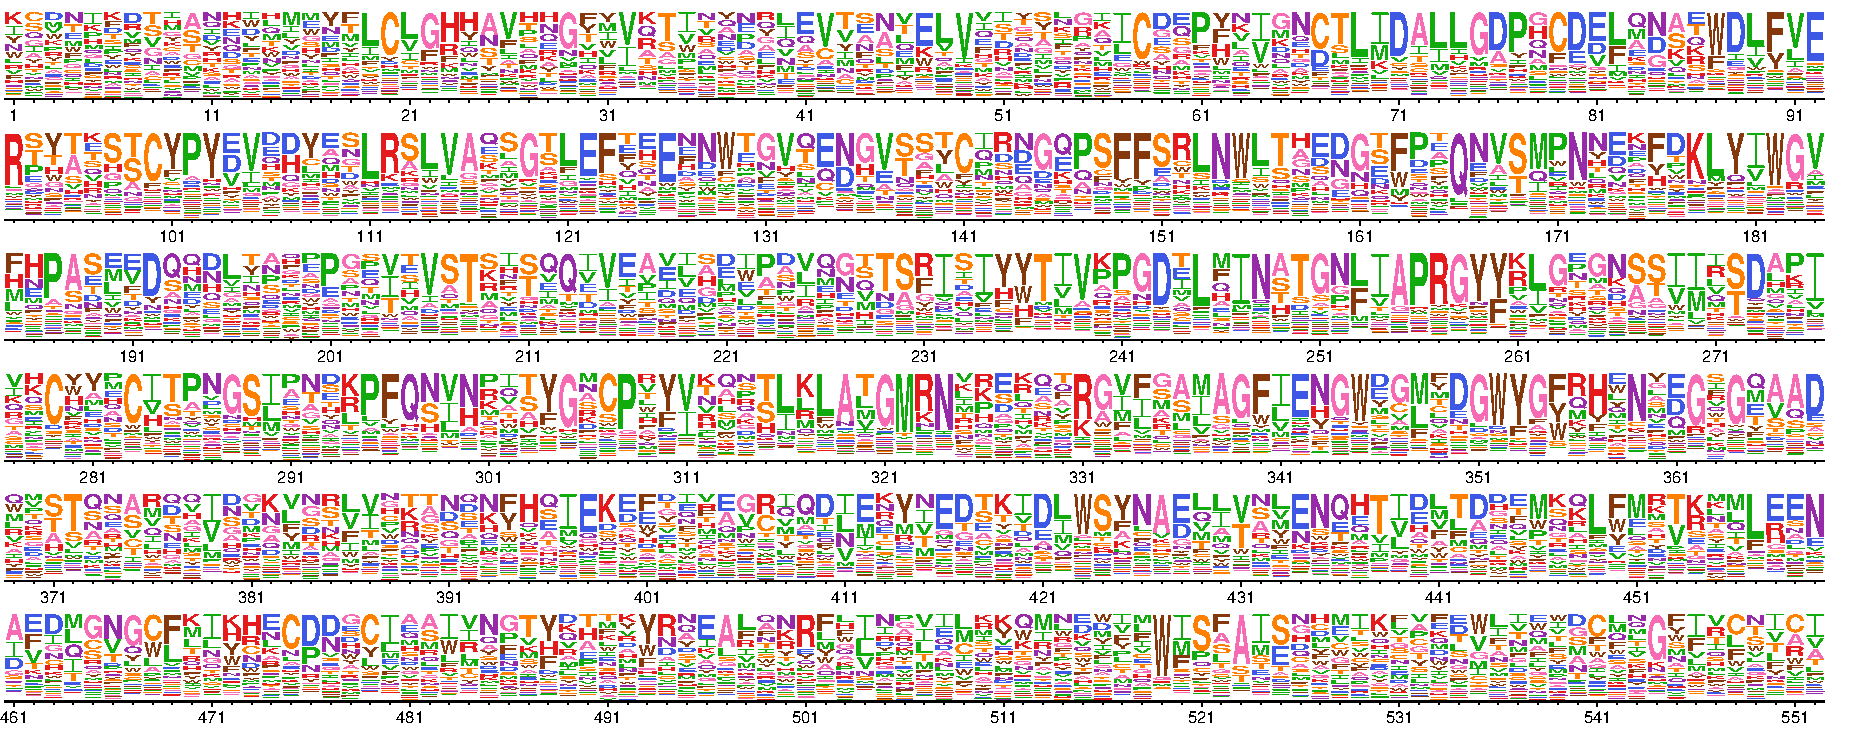
\includegraphics[width=\textwidth]{figures/prefs_lee}}
\caption{\label{suppfig:prefs_lee}
\textbf{H3 preferences measured by \textit{lee} rescaled with the ExpCM stringency parameter optimized in \ref{fig:tree_lee}A  ($\beta = 1.46$)}
\skhcomment{I need to change the $\beta$ value when the new \texttt{phydms} results finish running.} 
}
\end{suppfig}

\begin{suppfig}[H]
\centerline{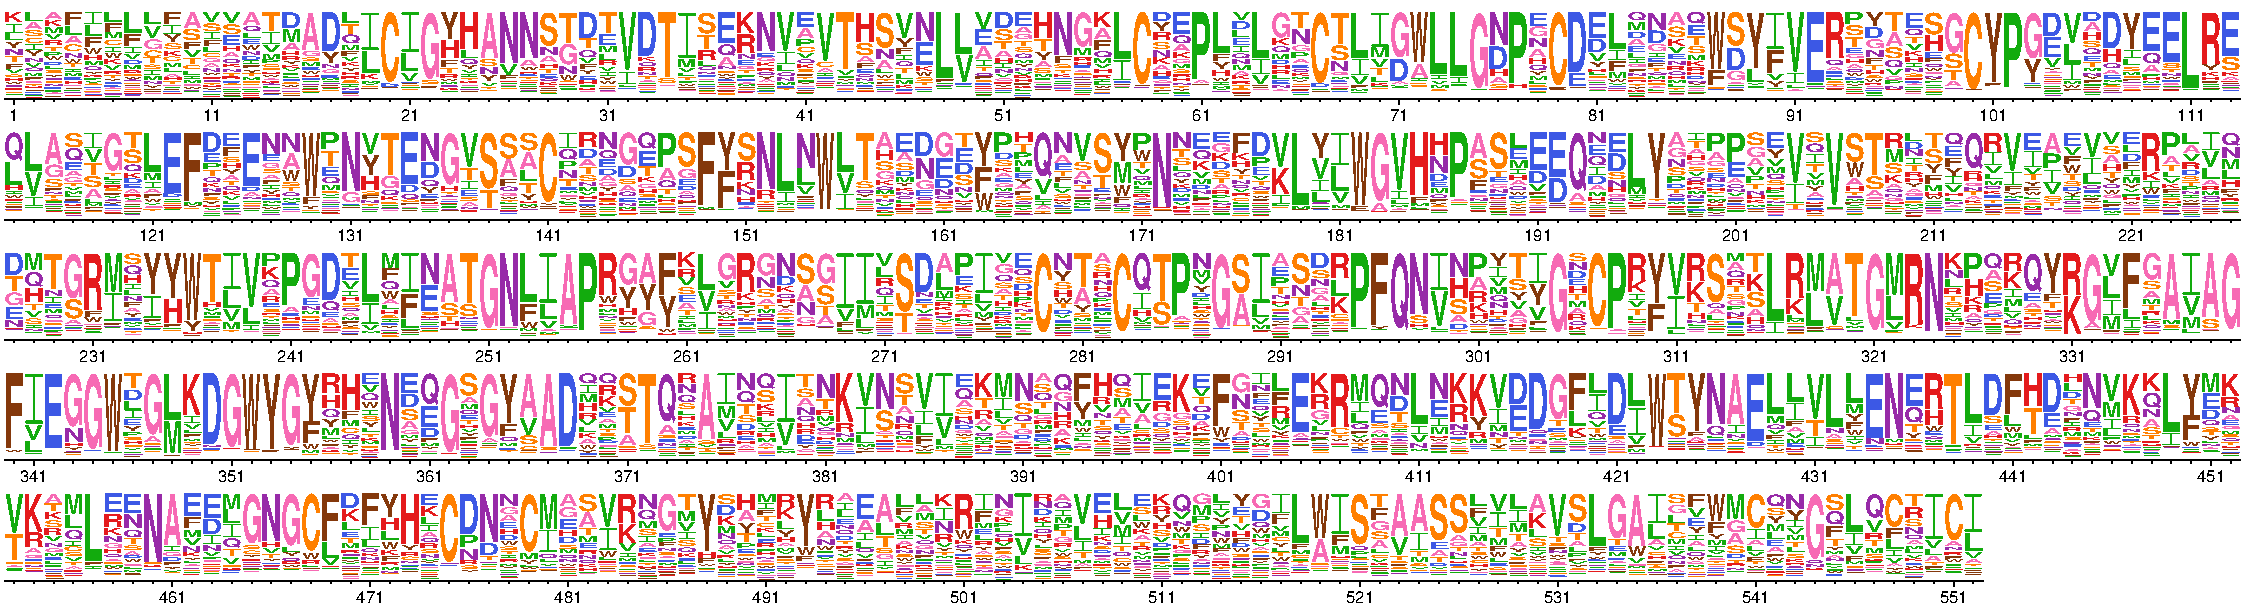
\includegraphics[width=\textwidth]{figures/prefs_average}}
\caption{\label{fig:prefs_average}
\textbf{The average of the H1 preferences measured by \cite{doud2016accurate} and the H3 preferences measured by \textit{Lee} rescaled with the ExpCM stringency parameter optimized in \ref{fig:tree_average}A  ($\beta = 1.77$)}}
\skhcomment{I need to change the $\beta$ value when the new \texttt{phydms} results finish running.}
\end{suppfig}
 


\begin{table}[t!]
\caption{\label{tab:simulation_params}
ExpCM parameters used to simulate sequences in Fig.~\ref{fig:simulation}.}
      \begin{tabular}{ccccc}
        \hline
          Parameter & Value\\ \hline
       	$\beta$ & $1.54$\\
	$\kappa$ & $3.60$\\
	$\omega$ & $0.20$\\
	$\phi_A$, $\phi_C$, $\phi_G$& $0.38$, $0.17$, $0.23$\\
      \end{tabular}
\end{table}

\begin{table}[t!]
\caption{\label{tab:wsn_low_params}
Model parameters used in  Fig.~\ref{fig:decay}.}
      \begin{tabular}{ccccc}
        \hline
          Model & Parameters\\ \hline
          ExpCM & $\beta=1.54196$\\
           & $\kappa=3.47184$\\
           & $\omega=0.219225$\\ 
          YNGKP M0 & $\kappa=2.9984$\\
          & $\omega=0.09076$\\
          YNGKP M5 & $\kappa=2.9984$\\
          & $\omega=0.09076$\\
      \end{tabular}
\end{table}

\begin{suppfig}[H]
\centerline{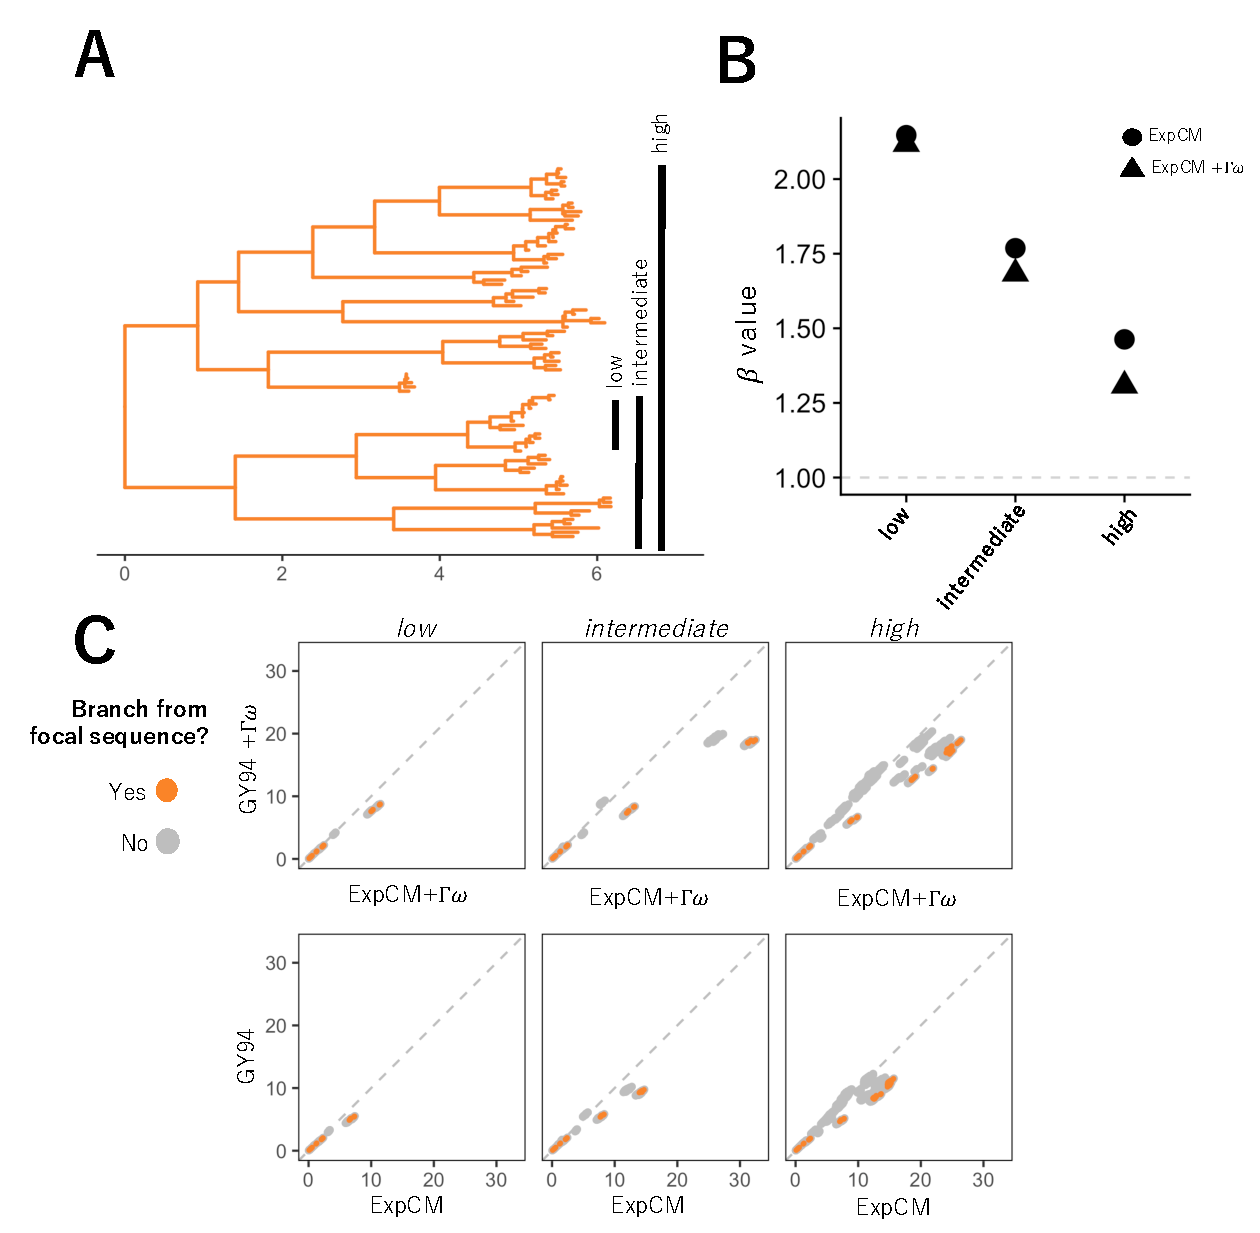
\includegraphics[width=0.85\textwidth]{figures/lee_compete}}
\caption{\label{fig:lee_compete}
\textbf{The ExpCM defined by H1 preferences lengthen longer branches on the HA tree.} 
\textbf{(A)} An HA alignment was subsampled to create three smaller alignments with varying degrees of divergence from the focal H3 sequence, referred to as "low", "intermediate", and "high". 
\textbf{(B)} The phylogenetic tree of the "high" alignment. 
The colors denote the alignment and the black circle denotes the focal H3 sequence. 
\textbf{(C)} The value of the ExpCM and ExpCM+$\Gamma\omega$ stringency parameter $\beta$ decreases as the divergence from the focal H3 sequence increases. 
\textbf{(D)} Comparisons of branch lengths optimized by the four substitution models for the varying degrees of divergence. 
Black points represent branches from the focal H3 sequence and grey points represent all other branches.  
The branch lengths are in average number of codon substitutions per site. 
}
\end{suppfig}


\clearpage 
\bibliographystyle{mbe}
\bibliography{references.bib}



\end{document}